%% ---------------------------------------------------------------------------
%% Rethinking Evaluation for Data-Driven Flood Early Warning
%% IEEE conference format (IEEEtran). Compile with pdflatex:
%%     pdflatex main && pdflatex main
%% Figures are generated by ../paper/make_figures.py into paper/figures/.
%% Placeholders are marked with \placeholder{} and MUST be replaced before
%% submission -- each one names the artefact that produces it.
%% ---------------------------------------------------------------------------
\documentclass[conference]{IEEEtran}
\IEEEoverridecommandlockouts

\usepackage{cite}
\usepackage{amsmath,amssymb}
\usepackage{graphicx}
\usepackage{booktabs}
\usepackage{multirow}
\usepackage{url}
\usepackage{xcolor}
\usepackage{tikz}
\usetikzlibrary{positioning,arrows.meta,fit,backgrounds}
\usepackage[hidelinks]{hyperref}

\graphicspath{{figures/}}

%% A visible, sized stand-in for artefacts that need data not in this repo.
\newcommand{\placeholder}[2]{%
  \fbox{\parbox[c][#1][c]{0.96\linewidth}{\centering\footnotesize
  \textcolor{red}{\textbf{PLACEHOLDER}}\\[2pt]#2}}}

\begin{document}

\title{Rethinking Evaluation for Data-Driven Flood\\Early Warning: Evidence from a
51-Node River\\Network in Sri Lanka}

%% Note: a line beginning with "[" directly after \\ is parsed as an optional
%% length argument, so each bracketed placeholder is wrapped in braces.
\author{\IEEEauthorblockN{{[Author Name]}}
\IEEEauthorblockA{\textit{{[Department]}} \\
\textit{{[Institution]}}\\
{[City]}, Sri Lanka \\
{[email]}}
}

\maketitle

\begin{abstract}
Data-driven flood early-warning systems are typically reported with a single
threshold-free ranking metric, and increasingly reach high scores. We show, on a
purpose-built national dataset for Sri Lanka, that such scores can be almost
entirely uninformative about operational skill. We release a leakage-controlled
daily panel of 51 gauged river nodes across 16 basins (2003--2024;
$409{,}350$ supervised node-days; 1{,}469 flood episodes) with a directed river
graph, and evaluate a multimodal transformer (MMF-Net) against four baselines
under three block protocols. Three findings follow. First, the standard target
--- next-day discharge above a per-node 98th percentile --- is close to
self-answering: a single-feature discharge-percentile rule attains PR-AUC
$0.8164$ and gradient-boosted trees $0.8496$, above our best network's $0.8355$.
Second, replacing the block-temporal split with a random split raises PR-AUC from
$0.704$ to $0.905$ while pre-onset event detection \emph{collapses} from
$0.380$ to $0.089$: leakage does not merely inflate the score, it selects a
different model that never warns before onset. Third, focal loss --- near
universal in imbalanced remote-sensing work --- is a defect rather than a
trade-off here, costing $0.0509$ PR-AUC and tripling calibration error at
identical architecture and seeds. We also report two independent null results for
a Sentinel-1 SAR branch. We argue that flood-forecasting benchmarks should report
event-level detection at a capped false-alarm ratio together with calibration,
and we release the dataset, code and evaluation harness.
\end{abstract}

\begin{IEEEkeywords}
flood early warning, evaluation protocol, data leakage, calibration, tabular deep
learning, graph neural networks, Sri Lanka
\end{IEEEkeywords}

%% ===========================================================================
\section{Introduction}

Sri Lanka's exposure to riverine flooding is severe and increasing. Over
1975--2025, cyclonic disturbance frequency rose from 1.3 to 4.1 systems per year
($+216\%$, Sen's slope $+0.73$/decade, $p<0.001$), extreme rainfall intensity
increased by $12.2$~mm/decade, and major flood events increased 4.5-fold
\cite{partheepan2026}. Cyclone Ditwah (November 2025) caused $620+$ deaths and
displaced approximately 1.1~million people across 21 districts --- the deadliest
cyclone-related event since the 2004 tsunami \cite{partheepan2026}.

Critically, the same study reports that forecast lead time has already improved
roughly six-fold (from 12--24~h to 120--168~h) while evacuation completion times
have remained static at 18--36~h, and that the correlation between forecast
accuracy and reduced casualties is weak ($R^2 < 0.4$) \cite{partheepan2026}. The
binding constraint is therefore not raw lead time. It is the translation of a
forecast into action --- a chain that breaks when warnings are generic,
uncalibrated, or issued so often that they are discounted.

This reframes what a useful flood model must deliver. It is not a higher ranking
score. It is a \emph{calibrated probability}, at a \emph{controlled false-alarm
rate}, \emph{before} an episode begins. Our central claim is that the metrics in
common use do not measure any of those three things, and that this is
demonstrable rather than rhetorical.

\textbf{Contributions.}
\begin{enumerate}
  \item A public, leakage-controlled spatiotemporal dataset for Sri Lanka: 51
        gauged nodes, 16 basins, daily 2003--2024, $409{,}350$ supervised
        node-days, 1{,}469 labelled flood episodes, with a directed river-flow
        graph and three precomputed block protocols (Section~\ref{sec:data}).
  \item Evidence that the conventional next-day threshold target is dominated by
        discharge persistence, so that PR-AUC on it is a ceiling rather than a
        contest (Section~\ref{sec:baselines}).
  \item A measured demonstration that random splitting selects a model that
        \emph{cannot} warn before onset, with event detection falling by 77\%
        while the headline score rises 29\% (Section~\ref{sec:leakage}).
  \item A clean negative result for focal loss, and two independent null results
        for a Sentinel-1 SAR branch (Sections~\ref{sec:ladder},
        \ref{sec:sar}).
  \item An evaluation protocol --- event-level detection at matched false-alarm
        ratio, with calibration reported alongside --- together with an open
        harness that implements it (Section~\ref{sec:protocol}).
\end{enumerate}

%% ===========================================================================
\section{Related Work}

\subsection{Deep learning for flood and streamflow forecasting}
LSTM rainfall--runoff modelling established that a single deep model trained
across many catchments can match or exceed calibrated conceptual hydrology
\cite{kratzert2018,kratzert2019}. Nearing \emph{et al.} extended this to
ungauged basins globally, reporting five-day-lead reliability comparable to or
better than same-day nowcasts from the Copernicus Global Flood Awareness System
\cite{nearing2024}. That result is directly relevant to us: our supervision
signal is derived from GloFAS reanalysis discharge \cite{harrigan2020}, a product
their system outperforms. We therefore position this work not as a competitor to
a global operational forecast, but as a national, node-level, fully reproducible
study of \emph{how such systems should be evaluated}.

\subsection{Graph neural networks on river networks}
Spatiotemporal GNNs have been applied to flood prediction using catchment graphs
\cite{kazadi2024,bentivoglio2025,taghizadeh2025}. The evidence that river
topology helps is contested. Kirschstein and Sun report that their model
``fails to benefit from the river network topology information, both on the
entire network and small subgraphs,'' with learned edge weights uncorrelated with
static topology \cite{kirschstein2024}. Wang \emph{et al.} reach the opposite
conclusion, but only after a reachability-based graph transformation that
mitigates over-squashing \cite{wang2025}. Our own graph-based family
(Section~\ref{sec:ladder}) is consistent with the former; we treat the question
as open and report it as such.

\subsection{Tabular deep learning}
Gradient-boosted trees remain strong on medium-sized tabular data
\cite{grinsztajn2022}. The published remedy is not depth but the input layer:
per-feature periodic embeddings substantially close the gap
\cite{gorishniy2022}. Our single largest gain reproduces this on a hydrological
panel (Section~\ref{sec:ladder}).

\subsection{Evaluation, leakage and calibration}
Roberts \emph{et al.} specify block cross-validation for temporally and spatially
structured data \cite{roberts2017}. Kapoor and Narayanan document leakage as a
reproducibility crisis across 17 fields, with a taxonomy of eight leakage types
\cite{kapoor2023}. Precision--recall analysis is preferred to ROC under strong
class imbalance \cite{davis2006,saito2015}, and POD/FAR/CSI are the standard
meteorological verification quantities \cite{jolliffe2012}. Modern networks are
badly calibrated by default; temperature scaling is the standard post-hoc remedy
\cite{guo2017}, and deep ensembles provide both accuracy and uncertainty
\cite{lakshminarayanan2017}.

\subsection{Sri Lankan flood prediction}
\label{sec:related-lk}
Prior Sri Lankan work is concentrated on single stations or single districts, and
--- crucially for this paper --- reports metrics that conceal the failure mode.
Table~\ref{tab:lk} summarises what the published numbers rest on.

Saubhagya \emph{et al.} forecast water level at Ratnapura (Kalu basin) with a
Bi-LSTM plus a GLS regression and ARIMA residual model, using six predictors over
2014--2019 \cite{saubhagya2025}. Their protocol is sound --- an expanding-window
temporal split --- and is the methodologically strongest local work. However,
their headline ``accuracies of 80\%, 80\% and 100\%'' for actionable events are
computed over the three Minor and two Critical events that occur in the whole
2017--2019 evaluation window; the Major class never occurs at all. Their reported
overall accuracy also sits at or below the majority-class rate in every year
(e.g.\ 92\% reported for 2019 against a 98.6\% ``never predict a flood'' rate).
They state explicitly that ``a better performance could have been achieved if
data from a higher number of nearby WL gauging stations were available''
\cite{saubhagya2025} --- the gap a national node network addresses.

Thilakarathne and Premachandra predict monthly flood occurrence for Anuradhapura
using ARIMA-forecast weather and an ANN classifier, reporting 91.7\% accuracy
under 10-fold cross-validation \cite{thilakarathne2017}. Their own table reports
mean recall $0.404$, with two of ten folds at precision $=$ recall $=0.000$.
Ten-fold cross-validation on a monthly time series is a random split, i.e.\
exactly the protocol characterised as invalid in \cite{roberts2017,kapoor2023}.

Mahaganapathy \emph{et al.} report a 99\% F1 score for Kalu Ganga catchments using
SMOTE and ensemble classifiers \cite{mahaganapathy2023}; the available abstract
does not state the splitting protocol.

Operationally, the Department of Irrigation issues basin warnings from observed
rainfall, catchment soil moisture, river water level and river trend
\cite{doi2024} --- a feature set our 33 dynamic channels deliberately mirror.
Official Kelani thresholds at the Nagalagam Street gauge are 5.0--7.0~ft (minor),
$>7.0$~ft (major) and $>9.0$~ft (dangerous) \cite{gunasekara2008}.

\begin{table}[t]
\caption{Scale and evidence base of prior Sri Lankan flood-prediction studies,
counted from each paper's own tables.}
\label{tab:lk}
\centering
\footnotesize
\begin{tabular}{@{}lcccc@{}}
\toprule
Study & Spatial units & Period & Resol. & Events eval. \\
\midrule
\cite{saubhagya2025} & 1 target $+$ 4 upstream & 2014--19 & daily & \textbf{5} \\
\cite{thilakarathne2017} & 1 district & 1976--2015 & monthly & 51 records \\
\cite{mahaganapathy2023} & 6 catchments & n/s & n/s & n/s \\
\textbf{This work} & \textbf{51 nodes / 16 basins} & \textbf{2003--24} & \textbf{daily} & \textbf{1{,}469} \\
\bottomrule
\end{tabular}
\end{table}

%% ===========================================================================
\section{Dataset and Problem Formulation}
\label{sec:data}

\subsection{Node network and graph}
We define 51 river nodes across 16 basins, each tagged with a climatic zone
(wet / intermediate / dry) and a network position (upstream / mid / downstream /
outlet). Fig.~\ref{fig:map} shows the network. The graph carries two
\emph{separately typed} relations that are never symmetrised: 35 directed
upstream$\rightarrow$downstream \emph{flow} edges curated from a
\texttt{downstream\_of} field, and 204 distance-decayed bidirectional
\emph{spatial} $k$-NN edges, plus self-loops. Edge attributes are
$[\,w,\ d_{\text{km}}/100,\ \Delta z/100,\ \mathbf{1}_{\text{flow}}\,]$, where
$\Delta z$ is the elevation drop from source to destination.

\begin{figure}[t]
\centering
\placeholder{4.6cm}{Study-area map: the 51 river nodes over Sri Lanka's basin
boundaries, coloured by climatic zone, with the 35 directed flow edges drawn.
\\[3pt]
\emph{Produce from} \texttt{data/processed/nodes.csv} \emph{and}
\texttt{edges.csv} \emph{with a basin shapefile (GADM level~2 or Survey Dept.
basin layer).}}
\caption{The 51-node river network. Node identity, basin, zone and position are
given in \texttt{scripts/common/nodes.py}.}
\label{fig:map}
\end{figure}

\subsection{Features and targets}
Each node-day carries 33 dynamic channels --- precipitation and multi-day
accumulations, an antecedent precipitation index, temperature, humidity, wind,
radiation, three soil-wetness depths with anomalies, and eight discharge-derived
channels --- plus 9 static terrain features. Heavy-tailed channels are
$\log(1+x)$ transformed before standardisation. Sources are NASA POWER
(meteorology), GloFAS via Open-Meteo (discharge) \cite{harrigan2020}, ERA5-Land
\cite{munoz2021} and Copernicus DEM.

The primary target is
\begin{equation}
y_{n,t} = \mathbf{1}\!\left[\, Q_{n,t+1} > \tau_n \,\right],\qquad
\tau_n = \mathrm{P}_{98}\!\left(Q_{n,\cdot}^{\text{train}}\right),
\end{equation}
i.e.\ next-day discharge at node $n$ exceeding that node's own 98th-percentile
threshold, with $\tau_n$ fitted on the training block only. Three auxiliary
classification heads (2-day, 3-day, and \emph{onset}, defined as a flood within
the horizon while not currently flooding) and two regression heads are trained
jointly. A \texttt{label\_confidence} weight in $[0.5,1]$ down-weights days
within $\pm15\%$ of $\tau_n$.

\subsection{Protocols}
\label{sec:protocol}
Random splitting is structurally impossible in this release: three block
protocols ship precomputed. The \emph{temporal} protocol trains on
$\le$2017-12-31, validates on 2018--2020 and tests on 2021 onward; the
\emph{basin} protocol holds out the entire Gin basin; the \emph{event} protocol
groups by episode identifier. A diagnostic random split exists solely to
\emph{measure} leakage (Section~\ref{sec:leakage}). All normalisation statistics,
percentile thresholds and day-of-year climatologies are fitted on the training
block alone. Table~\ref{tab:splits} gives the sizes.

\begin{table}[t]
\caption{Temporal protocol block sizes (valid supervised node-days).}
\label{tab:splits}
\centering
\footnotesize
\begin{tabular}{@{}lccc@{}}
\toprule
Block & Dates & $N$ & Positive rate \\
\midrule
Train & 2003-01-01 -- 2017-12-31 & 277{,}899 & 2.028\% \\
Val   & 2018-01-01 -- 2020-12-31 & \phantom{0}55{,}896 & 0.810\% \\
Test  & 2021-01-01 -- 2024-12-31 & \phantom{0}75{,}555 & 2.275\% \\
\midrule
Total & & 409{,}350 & \\
\bottomrule
\end{tabular}
\end{table}

The validation block is hydrologically quieter than train and test
(0.810\% vs 2.028\%/2.275\%). This is real hydrology, not a sampling artefact,
and it makes early stopping on node-day PR-AUC an optimistic-biased signal; we
therefore select on an episode-level criterion instead
(Section~\ref{sec:metrics}).

%% ===========================================================================
\section{Method}

\subsection{MMF-Net}
Fig.~\ref{fig:arch} shows the architecture. A batch is a set of \emph{days};
every forward pass sees the whole network, so that spatial variants are possible
without changing the data path.

Given a window $\mathbf{x}\in\mathbb{R}^{B\times L\times N\times F}$
($L=14$ days, $N=51$ nodes, $F=33$ channels) the nodes are folded into the batch
dimension and each scalar is given its own \emph{periodic--linear--ReLU} (PLR)
embedding \cite{gorishniy2022}: for feature $j$ with learned frequencies
$\mathbf{c}_j\in\mathbb{R}^{k}$,
\begin{equation}
\mathbf{e}_j(x)=\mathrm{ReLU}\!\left(\mathbf{W}_j
\big[\sin(2\pi\mathbf{c}_j x)\,\|\,\cos(2\pi\mathbf{c}_j x)\big]+\mathbf{b}_j\right).
\end{equation}
The motivation is precise: a linear layer applied to a raw scalar is monotone and
cannot represent a sharp decision boundary, which is exactly what a decision tree
obtains for free from a split point.

Per-day embeddings are concatenated, projected to one token per day, and pooled
by a \textsc{cls} token through a three-layer pre-LN transformer. A second,
cheaper attention block operates \emph{across} the 33 channels of the
time-averaged window, expressing conditional interactions (``this much rain
matters only when the soil is already wet'') that a single linear mixing layer
cannot. Static terrain then modulates the state by FiLM \cite{perez2018},
$\mathbf{h}\leftarrow\mathrm{LN}\!\left(\mathbf{h}\odot(1+\gamma)+\beta\right)$,
with the generator's output layer zero-initialised so the module begins as
exactly the identity. A fusion MLP and a shared head produce four classification
logits and two regressions.

\begin{figure}[t]
\centering
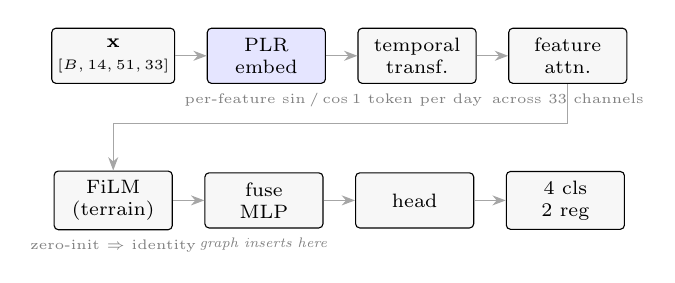
\begin{tikzpicture}[
  font=\scriptsize,
  box/.style={draw,rounded corners=1.5pt,align=center,minimum height=7mm,
              minimum width=15mm,inner xsep=2pt,fill=black!3},
  hl/.style={box,fill=blue!10},
  note/.style={font=\tiny,text=gray,align=center,inner sep=1pt},
  ar/.style={-{Stealth[length=1.7mm]},gray!70}
]
%% ---- row 1: the per-node encoder ----------------------------------------
\node[box]                        (in)  {$\mathbf{x}$\\{\tiny$[B,14,51,33]$}};
\node[hl,  right=4mm of in]       (plr) {PLR\\embed};
\node[box, right=4mm of plr]      (tt)  {temporal\\transf.};
\node[box, right=4mm of tt]       (fa)  {feature\\attn.};
\foreach \a/\b in {in/plr, plr/tt, tt/fa} \draw[ar] (\a) -- (\b);

\node[note, below=0.8mm of plr] {per-feature $\sin/\cos$};
\node[note, below=0.8mm of tt]  {1 token per day};
\node[note, below=0.8mm of fa]  {across 33 channels};

%% ---- row 2: conditioning, fusion, heads ---------------------------------
\node[box, below=11mm of in]      (film){FiLM\\(terrain)};
\node[box, right=4mm of film]     (fuse){fuse\\MLP};
\node[box, right=4mm of fuse]     (head){head};
\node[box, right=4mm of head]     (out) {4 cls\\2 reg};
\foreach \a/\b in {film/fuse, fuse/head, head/out} \draw[ar] (\a) -- (\b);

\node[note, below=0.8mm of film] {zero-init $\Rightarrow$ identity};
\node[note, below=0.8mm of fuse] {\textit{graph inserts here}};

%% wrap from the end of row 1 to the start of row 2
\draw[ar] (fa.south) -- ++(0,-5.0mm) -| (film.north);
\end{tikzpicture}
\caption{MMF-Net. Nodes are folded into the batch dimension, so the encoder is
per-node; the graph-based family of Section~\ref{sec:ladder} inserts relational
message passing between \emph{fuse} and \emph{head}. Parameter shares for the
$711$k headline model: temporal transformer $61.7\%$, feature attention
$19.4\%$, head $9.3\%$, fusion $7.0\%$, FiLM $2.5\%$.}
\label{fig:arch}
\end{figure}

\subsection{Training, calibration and thresholding}
All heads are optimised jointly with a masked weighted sum of per-head binary
cross-entropy plus a Huber term for the regressions. Optimisation is AdamW,
$\mathrm{lr}=10^{-3}$, cosine schedule with five warmup epochs, 60 epochs with
early stopping (patience 10). Five seeds are trained independently and their
logits averaged \cite{lakshminarayanan2017}; a single temperature is then fitted
\emph{on validation} \cite{guo2017} and the decision threshold is likewise chosen
on validation and frozen. The test block is touched once.

\subsection{Metrics}
\label{sec:metrics}
We report PR-AUC \cite{davis2006,saito2015}, Brier score, expected calibration
error, and POD/FAR/CSI \cite{jolliffe2012}. The operationally decisive quantity
is \emph{pre-onset event detection} (\texttt{ev.det}): the fraction of flood
episodes for which the model raises an alarm in the seven days \emph{before}
onset, with mean lead time among detected episodes. Model selection uses an
episode-level PR-AUC in which each episode contributes one positive, scored by
the model's maximum probability in the pre-onset window, and each flood-free
node-week contributes one negative.

%% ===========================================================================
\section{Results}

\subsection{Baselines: the target is close to self-answering}
\label{sec:baselines}
Table~\ref{tab:baselines} gives four reference models under the temporal
protocol. The decisive row is \texttt{discharge\_pctl}: a single feature, no
learning, PR-AUC $0.8164$. Because the target is next-day discharge above a
percentile and discharge is strongly autocorrelated, today's percentile nearly
answers the question. Gradient-boosted trees add only $0.033$ on top of that.

\begin{table}[t]
\caption{Baselines, temporal protocol, test block.}
\label{tab:baselines}
\centering
\footnotesize
\begin{tabular}{@{}lccccc@{}}
\toprule
Baseline & PR-AUC & ROC-AUC & POD & FAR & \texttt{ev.det} \\
\midrule
Persistence          & 0.5900 & 0.882 & 0.769 & 0.231 & 0.223 \\
Climatology          & 0.1080 & 0.870 & 0.556 & 0.882 & 0.515 \\
Discharge percentile & 0.8164 & 0.984 & 0.769 & 0.231 & 0.223 \\
\textbf{GBT (LightGBM)} & \textbf{0.8496} & 0.988 & 0.634 & 0.080 & 0.161 \\
\bottomrule
\end{tabular}
\end{table}

The consequence is that PR-AUC on this target measures persistence more than
skill, and that the genuine headroom lies elsewhere: the best baseline warns
before onset on only 22.3\% of episodes, and the strongest baseline (GBT) on
16.1\%. Climatology's apparently high $0.515$ is an artefact of alarming almost
constantly (FAR $0.882$), which is precisely the confound
Section~\ref{sec:opp} addresses.

\subsection{Ablation ladder}
\label{sec:ladder}
Table~\ref{tab:ladder} and Fig.~\ref{fig:ladder} give the MMF-Net ladder, each
rung changing exactly one thing.

\begin{table}[t]
\caption{MMF-Net ablation ladder, temporal protocol, test block. $\times5$
denotes a five-seed ensemble with temperature scaling.}
\label{tab:ladder}
\centering
\footnotesize
\begin{tabular}{@{}lccccr@{}}
\toprule
Rung & Change & PR-AUC & \texttt{ev.det} & FAR & Params \\
\midrule
N0 & linear embeddings      & 0.6083 & 0.290 & 0.412 & 551k \\
N1 & $+$ PLR embeddings     & \textbf{0.7605} & 0.420 & 0.325 & 555k \\
N2 & $+$ feature attention  & 0.7738 & \textbf{0.423} & 0.313 & 693k \\
N3 & $+$ FiLM terrain       & 0.8269 & 0.197 & 0.110 & 711k \\
N4 & $+$ focal loss         & 0.7592 & 0.220 & 0.138 & 711k \\
N5$\times5$ & $+$ ensemble (focal) & 0.7846 & 0.208 & 0.145 & 711k \\
\textbf{N5\_bce}$\times5$ & \textbf{the same, BCE} & \textbf{0.8355} & 0.220 & 0.120 & 711k \\
\midrule
N6\_sc$\times5$  & $+$ SAR scalars   & 0.7284 & 0.397 & 0.344 & 719k \\
N6\_gat$\times5$ & $+$ gated SAR CNN & 0.8310 & 0.217 & 0.107 & 11{,}967k \\
\bottomrule
\end{tabular}
\end{table}

\begin{figure}[t]
\centering
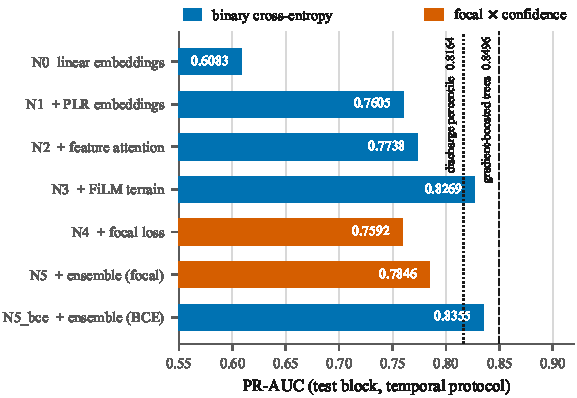
\includegraphics[width=\linewidth]{fig_ladder.pdf}
\caption{PR-AUC up the ladder. The two reference lines are the
discharge-percentile rule and gradient-boosted trees. Bars are coloured by loss
function: the focal-loss rungs (N4, N5) form a visible regression that reverting
to BCE removes.}
\label{fig:ladder}
\end{figure}

\textbf{The input layer, not depth, closes the gap to trees.} N0$\rightarrow$N1
changes only the numerical embedding and moves PR-AUC by $+0.152$ --- the largest
single-change gain in the study, and larger than terrain conditioning
($+0.105$ in our graph-based family). This reproduces \cite{gorishniy2022} on a
hydrological panel and supports the diagnosis of \cite{grinsztajn2022}.

\textbf{Focal loss is a defect, not a trade-off.} N5$\rightarrow$N5\_bce changes
\emph{only} the loss --- identical architecture, seeds, ensemble and calibrator
--- and gains $+0.0509$ PR-AUC while reducing ECE from $0.0043$ to $0.0016$; the
single-seed comparison N3 (BCE, ECE $0.0032$) against N4 (focal, ECE $0.0525$) is
starker still. Given the ubiquity of focal loss \cite{lin2017} in imbalanced
geoscience pipelines, we report this as a transferable negative result.

\textbf{The best network still loses to trees.} N5\_bce reaches $0.8355$ against
the GBT's $0.8496$ --- best in the study on PR-AUC, ECE ($0.0016$), Brier
($0.0080$), CSI ($0.561$) and F1 ($0.719$), at 711k parameters, but $0.0141$
short of a gradient-boosted tree and only $0.019$ above a one-line percentile
rule.

\subsection{Differences at the top are inside seed noise}
Across N5\_bce's five seeds, best-validation episode PR-AUC ranged
$0.3375$--$0.3856$, a spread of $0.0481$. Fig.~\ref{fig:seed} places the
differences being ranked against that spread: the N5\_bce--N6\_gated
($0.0045$) and N5\_bce--N3 ($0.0086$) gaps are well inside it, whereas the
loss effect ($0.0509$) clears it. We therefore claim the loss result and
explicitly \emph{decline} to claim an ordering among the top three
configurations.

\begin{figure}[t]
\centering
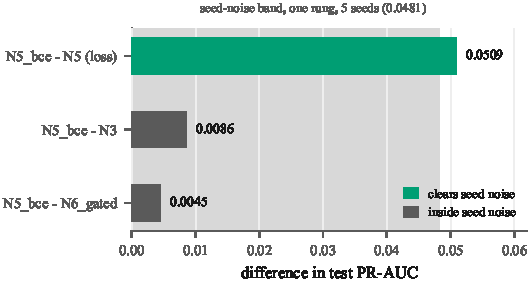
\includegraphics[width=\linewidth]{fig_seed_noise.pdf}
\caption{Differences between configurations against the seed-to-seed spread of a
single configuration. Only the loss effect is resolvable by this experiment.}
\label{fig:seed}
\end{figure}

\subsection{Leakage selects a different model}
\label{sec:leakage}
Table~\ref{tab:protocols} and Fig.~\ref{fig:leakage} report one architecture
under three protocols, with every hyperparameter held fixed.

\begin{table}[t]
\caption{One model, three protocols. The random split is diagnostic only.}
\label{tab:protocols}
\centering
\footnotesize
\begin{tabular}{@{}lccccc@{}}
\toprule
Protocol & PR-AUC & Brier & POD & FAR & \texttt{ev.det} \\
\midrule
Block temporal & 0.704 & 0.0135 & 0.621 & 0.342 & \textbf{0.380} \\
Basin holdout  & 0.840 & 0.0078 & 0.498 & 0.081 & 0.217 \\
\textbf{Random} & \textbf{0.905} & 0.0051 & 0.753 & 0.113 & \textbf{0.089} \\
\bottomrule
\end{tabular}
\end{table}

\begin{figure}[t]
\centering
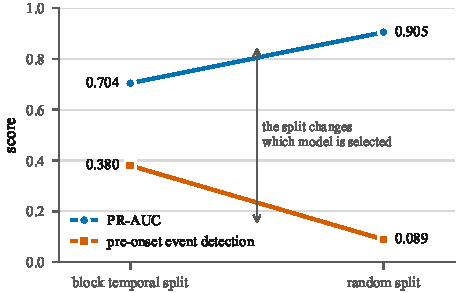
\includegraphics[width=\linewidth]{fig_leakage.pdf}
\caption{The same architecture under a block-temporal and a random split. PR-AUC
rises 29\% relative while pre-onset event detection falls 77\%. A study reporting
only the former would conclude the random-split model is far better; it is in
fact operationally useless.}
\label{fig:leakage}
\end{figure}

Under a random split PR-AUC rises from $0.704$ to $0.905$ ($+29\%$ relative),
above the GBT baseline and above every honest configuration we trained. Its
pre-onset event detection simultaneously \emph{collapses} from $0.380$ to
$0.089$. The random-split model has learned to interpolate between neighbouring
days --- days that are, under that protocol, in the training set --- and has
stopped forecasting altogether.

That PR-AUC is inflated by leakage is known \cite{roberts2017,kapoor2023}. The
contribution here is the second half: leakage does not merely add a bias to a
score, it \emph{changes which model is selected}, in the direction that destroys
operational value. Any pipeline selecting on a leaked ranking metric will
systematically prefer the model that cannot warn.

We note that the basin-holdout row is \emph{not} comparable to the temporal row:
that protocol still trains on the full 2003--2024 span and so retains temporal
leakage by construction. It measures spatial transfer only, and its $0.840$
should never be quoted as this study's best result.

\subsection{Operating points, not models}
\label{sec:opp}
Fig.~\ref{fig:operating} plots detection against false-alarm ratio for every
configuration. FAR spans $0.080$ to $0.882$. Reading \texttt{ev.det} down a
results column therefore compares thresholds rather than models: N2's
$0.423$ at FAR $0.313$ and N3's $0.197$ at FAR $0.110$ are not a regression in
skill but a move along an operating curve, and N3's threshold-free PR-AUC in fact
\emph{rose}. We supply an offline utility that re-derives every threshold to a
common false-alarm budget, and we recommend that flood papers report detection at
a stated FAR rather than at each model's own optimum.

\begin{figure}[t]
\centering
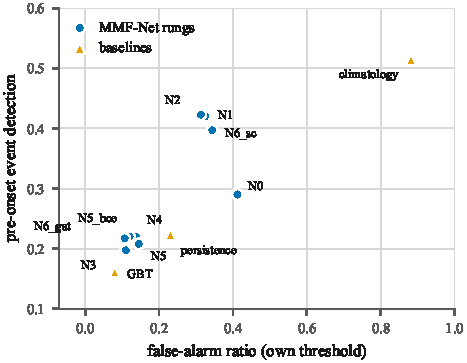
\includegraphics[width=\linewidth]{fig_operating_points.pdf}
\caption{Pre-onset event detection against false-alarm ratio at each model's own
validation-chosen threshold. The spread in FAR is why the detection column of a
results table is not comparable down the page.}
\label{fig:operating}
\end{figure}

\subsection{Calibration}
The ensemble plus temperature scaling reduces expected calibration error to
$0.0016$ for N5\_bce, against $0.0525$ for the uncalibrated focal-loss rung.
Fig.~\ref{fig:reliability} gives the reliability diagram.

\begin{figure}[t]
\centering
\placeholder{4.2cm}{Reliability diagram for N5\_bce with 15 equal-count bins,
plus the uncalibrated focal rung N4 for contrast; inset histogram of predicted
probabilities.
\\[3pt]
\emph{Produce from} \texttt{runs/N5\_bce\_temporal\_preds.npz} \emph{using}
\texttt{floodlib.metrics.reliability\_curve}.}
\caption{Calibration of the headline model after temperature scaling.}
\label{fig:reliability}
\end{figure}

\subsection{The SAR branch does not help}
\label{sec:sar}
A Sentinel-1 branch was evaluated twice. In our graph-based family a ResNet-18
embedding concatenated into the fusion input was null. In MMF-Net, a pretrained
encoder fused through a learned gate (zero-initialised with a negative bias, so
the module begins closed) reached $0.8310$ with $11{,}967$k parameters ---
\emph{below} the $711$k image-free model. What had appeared to be a vision gain
was the BCE loss recovering what focal loss had destroyed.

We report this as a \emph{coverage} result rather than a claim about SAR for
flood mapping in general \cite{bonafilia2020}: imagery reaches only 9 of 51
nodes, and Sentinel-1's $\sim$12-day revisit is structurally mismatched to a
one-day horizon. Lead time in this system must come from the daily meteorological
and discharge channels.

%% ===========================================================================
\section{Discussion}

Three practical recommendations follow.

\textbf{Report event-level detection at a capped false-alarm ratio.} A
threshold-free ranking metric on a next-day threshold target is dominated by
persistence, and a detection rate at each model's own optimum is not comparable
across models. Neither supports an operational decision.

\textbf{Report calibration alongside.} The evidence from
\cite{partheepan2026} is that the binding constraint in Sri Lanka is
warning-to-action, and that over-frequent or discounted warnings break that
chain. A probability that is right on average at every confidence level is
therefore not a nicety.

\textbf{Treat the split as part of the model.} Our random-split configuration
would, on the usual headline metric, be reported as the best model in this paper.
It is the worst. Because a leaked protocol changes model \emph{selection}, no
amount of downstream metric care compensates for it.

%% ===========================================================================
\section{Limitations}

\emph{No embargo between blocks.} The 14-day lookback is indexed absolutely, so
test days in the first 13 days of 2021 read features from December 2020, which
lies in the validation block. This is causal and not label leakage, but it is
uncontrolled and a 13-day embargo would remove it.

\emph{Same nodes in train and test.} The temporal protocol evaluates the same 51
gauges at later dates. Spatial transfer is measured only by the Gin-basin
holdout, on 3 nodes, and in our graph-based family alone.

\emph{Labels are model-derived.} Supervision comes from GloFAS reanalysis
discharge \cite{harrigan2020}, not from gauge observations or inundation records;
episodes were cross-checked against documented events but the label is a
reanalysis product with its own biases. Nearing \emph{et al.} report outperforming
GloFAS \cite{nearing2024}, which bounds what a model fitted to it can mean.

\emph{Single-seed rungs.} N0--N4 are single seeds; given the measured spread of
$0.0481$, individual rung-to-rung differences below roughly $0.02$ PR-AUC should
not be read as orderings.

\emph{RQ on river topology unresolved.} Whether directed flow edges help is not
settled by this study, consistent with the disagreement between
\cite{kirschstein2024} and \cite{wang2025}. An encoder-matched comparison is in
progress.

%% ===========================================================================
\section{Conclusion}

On a national, leakage-controlled dataset for Sri Lanka we find that the metric
conventions of data-driven flood forecasting can be actively misleading: the
usual target is dominated by discharge persistence, the usual splitting protocol
selects models that never warn before onset, and a widely used imbalance loss is
a net regression. Our best network is genuinely well calibrated and compact but
does not beat gradient-boosted trees on the headline score --- and we argue that
this is the correct thing to report, because the headline score is not the thing
that matters. We release the dataset, the models and an evaluation harness that
implements event-level detection at matched false-alarm ratio, so that subsequent
work on this basin network is comparable by construction.

\section*{Reproducibility}
Dataset, model code, preset ladders and evaluation harness:
\texttt{[repository URL]}. All results in this paper are produced by
\texttt{models/kaggle\_run.py} and rendered by \texttt{models/results\_doc.py};
figures are generated by \texttt{paper/make\_figures.py}.

\section*{Acknowledgment}
Weather and soil-wetness variables from the NASA POWER project (LaRC,
MERRA-2/GEOS). River discharge from GloFAS, Copernicus Emergency Management
Service, delivered via Open-Meteo (CC-BY 4.0). Sentinel-1 RTC and Copernicus DEM
via Microsoft Planetary Computer. Flood-episode validation used public reporting
from the Sri Lanka Disaster Management Centre and ReliefWeb.

%% ===========================================================================
\begin{thebibliography}{00}

\bibitem{partheepan2026} K. Partheepan, M. M. Musthafa, T. Bhavan, S. Acharjee,
and B. Nath, ``Analysis and risk evolution of floods and cyclones in Sri Lanka
from 1975 to 2025 towards resilient strategies,'' \emph{Discover Geoscience},
vol. 4, no. 168, 2026.

\bibitem{kratzert2018} F. Kratzert, D. Klotz, C. Brenner, K. Schulz, and
M. Herrnegger, ``Rainfall--runoff modelling using Long Short-Term Memory (LSTM)
networks,'' \emph{Hydrol. Earth Syst. Sci.}, vol. 22, pp. 6005--6022, 2018.

\bibitem{kratzert2019} F. Kratzert \emph{et al.}, ``Towards learning universal,
regional, and local hydrological behaviors via machine learning applied to
large-sample datasets,'' \emph{Hydrol. Earth Syst. Sci.}, vol. 23,
pp. 5089--5110, 2019.

\bibitem{nearing2024} G. Nearing \emph{et al.}, ``Global prediction of extreme
floods in ungauged watersheds,'' \emph{Nature}, vol. 627, pp. 559--563, 2024.

\bibitem{harrigan2020} S. Harrigan \emph{et al.}, ``GloFAS-ERA5 operational
global river discharge reanalysis 1979--present,'' \emph{Earth Syst. Sci. Data},
vol. 12, pp. 2043--2060, 2020.

\bibitem{munoz2021} J. Mu\~{n}oz-Sabater \emph{et al.}, ``ERA5-Land: a
state-of-the-art global reanalysis dataset for land applications,'' \emph{Earth
Syst. Sci. Data}, vol. 13, pp. 4349--4383, 2021.

\bibitem{kazadi2024} A. Kazadi \emph{et al.}, ``FloodGNN-GRU: a spatio-temporal
graph neural network for flood prediction,'' \emph{Environmental Data Science},
2024.

\bibitem{bentivoglio2025} R. Bentivoglio \emph{et al.}, ``Multi-scale hydraulic
graph neural networks for flood modelling,'' \emph{Nat. Hazards Earth Syst.
Sci.}, vol. 25, p. 335, 2025.

\bibitem{taghizadeh2025} M. Taghizadeh \emph{et al.}, ``Interpretable
physics-informed graph neural networks for flood forecasting,''
\emph{Computer-Aided Civil and Infrastructure Engineering}, vol. 40, no. 18,
pp. 2629--2649, 2025.

\bibitem{kirschstein2024} N. Kirschstein and Y. Sun, ``The merit of river network
topology for neural flood forecasting,'' in \emph{Proc. ICML}, 2024.

\bibitem{wang2025} Y. Wang \emph{et al.}, ``Accelerating flood warnings by 10
hours: the power of river network topology in AI-enhanced flood forecasting,''
\emph{npj Natural Hazards}, vol. 2, no. 45, 2025.

\bibitem{grinsztajn2022} L. Grinsztajn, E. Oyallon, and G. Varoquaux, ``Why do
tree-based models still outperform deep learning on typical tabular data?,'' in
\emph{Proc. NeurIPS}, 2022.

\bibitem{gorishniy2022} Y. Gorishniy, I. Rubachev, and A. Babenko, ``On
embeddings for numerical features in tabular deep learning,'' in \emph{Proc.
NeurIPS}, 2022.

\bibitem{roberts2017} D. R. Roberts \emph{et al.}, ``Cross-validation strategies
for data with temporal, spatial, hierarchical, or phylogenetic structure,''
\emph{Ecography}, vol. 40, no. 8, pp. 913--929, 2017.

\bibitem{kapoor2023} S. Kapoor and A. Narayanan, ``Leakage and the
reproducibility crisis in machine-learning-based science,'' \emph{Patterns},
vol. 4, no. 9, p. 100804, 2023.

\bibitem{davis2006} J. Davis and M. Goadrich, ``The relationship between
precision-recall and ROC curves,'' in \emph{Proc. ICML}, 2006, pp. 233--240.

\bibitem{saito2015} T. Saito and M. Rehmsmeier, ``The precision-recall plot is
more informative than the ROC plot when evaluating binary classifiers on
imbalanced datasets,'' \emph{PLOS ONE}, vol. 10, no. 3, p. e0118432, 2015.

\bibitem{jolliffe2012} I. T. Jolliffe and D. B. Stephenson, Eds., \emph{Forecast
Verification: A Practitioner's Guide in Atmospheric Science}, 2nd ed. Chichester,
U.K.: Wiley, 2012.

\bibitem{guo2017} C. Guo, G. Pleiss, Y. Sun, and K. Q. Weinberger, ``On
calibration of modern neural networks,'' in \emph{Proc. ICML}, 2017.

\bibitem{lakshminarayanan2017} B. Lakshminarayanan, A. Pritzel, and C. Blundell,
``Simple and scalable predictive uncertainty estimation using deep ensembles,''
in \emph{Proc. NeurIPS}, 2017.

\bibitem{lin2017} T.-Y. Lin, P. Goyal, R. Girshick, K. He, and P. Doll\'{a}r,
``Focal loss for dense object detection,'' in \emph{Proc. ICCV}, 2017.

\bibitem{perez2018} E. Perez, F. Strub, H. de Vries, V. Dumoulin, and
A. Courville, ``FiLM: Visual reasoning with a general conditioning layer,'' in
\emph{Proc. AAAI}, 2018.

\bibitem{bonafilia2020} D. Bonafilia, B. Tellman, T. Anderson, and E. Issenberg,
``Sen1Floods11: a georeferenced dataset to train and test deep learning flood
algorithms for Sentinel-1,'' in \emph{Proc. IEEE/CVF CVPR Workshops}, 2020,
pp. 835--845.

\bibitem{saubhagya2025} S. Saubhagya, C. Tilakaratne, P. Lakraj, and
M. Mammadov, ``A fusion of deep learning and time series regression for flood
forecasting: an application to the Ratnapura area based on the Kalu river basin
in Sri Lanka,'' \emph{Forecasting}, vol. 7, no. 2, p. 29, 2025.

\bibitem{thilakarathne2017} H. Thilakarathne and K. Premachandra, ``Predicting
floods in North Central Province of Sri Lanka using machine learning and data
mining methods,'' in \emph{Proc. SLAAI Int. Conf. Artificial Intelligence}, 2017,
pp. 44--49.

\bibitem{mahaganapathy2023} A. Mahaganapathy, W. U. Wickramaarachchi, and
R. M. K. T. Rathnayaka, ``Flood prediction using machine learning based on
metrological and topographical features of Kalu Ganga river basin, Sri Lanka,''
in \emph{Proc. ASURS}, 2023, p. 28 (abstract).

\bibitem{gunasekara2008} I. P. A. Gunasekara, ``Flood hazard mapping in lower
reach of Kelani river,'' \emph{ENGINEER --- J. Inst. Engineers Sri Lanka},
vol. 41, no. 5, pp. 149--154, 2008.

\bibitem{doi2024} Department of Irrigation, Sri Lanka, ``Present flood
forecasting and warning practices: preparation for South-West monsoon,''
Ministry of Irrigation briefing, May 2024.

\end{thebibliography}

\end{document}
